\documentclass[12pt,letterpaper]{article}
\usepackage[utf8]{inputenc}
\usepackage[spanish]{babel}
\usepackage{graphicx}
\usepackage[left=2cm,right=2cm,top=2cm,bottom=2cm]{geometry}
\usepackage{graphicx} % figuras
% \usepackage{subfigure} % subfiguras
\usepackage{float} % para usar [H]
\usepackage{amsmath}
%\usepackage{txfonts}
\usepackage{stackrel} 
\usepackage{multirow}
\usepackage{enumerate} % enumerados
\renewcommand{\labelitemi}{$-$}
\renewcommand{\labelitemii}{$\cdot$}
% \author{}
% \title{Caratula}
\begin{document}

% Fancy Header and Footer
% \usepackage{fancyhdr}
% \pagestyle{fancy}
% \cfoot{}
% \rfoot{\thepage}
%

% \usepackage[hidelinks]{hyperref} % CREA HYPERVINCULOS EN INDICE

% \author{}
\title{Caratula}

\begin{titlepage}
\begin{center}
\large{UNERSIDAD PRIVADA DE TACNA}\\
\vspace*{-0.025in}
\begin{figure}[htb]
\begin{center}

\includegraphics[width=7cm]{./Imagenes/logo}
\end{center}
\end{figure}
\vspace*{0.15in}
INGENIERIA DE SISTEMAS  \\

\vspace*{0.3in}
\begin{large}
\textbf{TITULO:} \\
\end{large}

\vspace*{0.1in}
\begin{Large}
\textbf{Diseño de Indicadores} \\

\end{Large}

\vspace*{0.3in}
\begin{Large}
\textbf{CURSO:} \\
\end{Large}

\vspace*{0.1in}
\begin{large}
INTELIGENCIA DE NEGOCIOS\\
\end{large}

\vspace*{0.3in}
\begin{Large}
\textbf{DOCENTE(ING):} \\
\end{Large}

\vspace*{0.1in}
\begin{large}
 Patrick Cuadros Quiroga\\
\end{large}

\vspace*{0.4in}
\vspace*{0.1in}
\begin{large}
\textbf{INTEGRANTE:} \\
\begin{flushleft}
Zavala Venegas, Luis Angel	\hfill	(2010037899)\\
Condori Quiso, Jesus		\hfill	(2008032440)\\
Condori Tito, Hernan		\hfill	(2009034553)\\
Vilca Chambilla, Wilfredo		\hfill	(2006028540)\\
Vilca Mamani, Elisban		\hfill	(2013000787)

\centering  %CENTRA UN TEXTO
\vspace*{0.9in}
\begin{large}
Tacna\\ 29-10-2018
\end{large}


\end{flushleft}
\end{large}
\end{center}

\end{titlepage}


\tableofcontents % INDICE
\thispagestyle{empty} % INDICE SIN NUMERO
\newpage
\setcounter{page}{1} % REINICIAR CONTADOR DE PAGINAS DESPUES DEL INDICE


\section{Introdución} 
\vspace{12mm} %5mm vertical space


Con la promulgación de la Ley No 30220, Ley Universitaria, el Ministerio de Educación (MINEDU) asume la rectoría de la Política de Aseguramiento de la Calidad de la Educación Superior Universitaria. Además, se crea la Superintendencia Nacional de Educación Superior Universitaria (SUNEDU), y se introduce el licenciamiento obligatorio y renovable de las universidades, en lugar de la autorización de funcionamiento provisional y definitiva del anterior marco legal.
El diseño del modelo de licenciamiento se enmarca en la Política de Aseguramiento de la Calidad de la
Educación Superior Universitaria. En ella, el licenciamiento, conjuntamente con la acreditación, el fomento y los sistemas de información, conforman los cuatro pilares del Sistema de Aseguramiento de la Calidad (SAC). En dicho sistema, el licenciamiento opera como un mecanismo de protección del bienestar individual y social al no permitir la existencia de un servicio por debajo de las condiciones básicas de calidad (en adelante, CBC).
En el marco del SAC, la acreditación y el licenciamiento se definen como procesos distintos, pero a su vez complementarios, de evaluación de la calidad. Mientras que la acreditación es voluntaria, el licenciamiento es un requisito obligatorio para el funcionamiento de las universidades. Además, las CBC del licenciamiento constituyen un primer nivel para ofrecer un servicio de calidad, mientras que la acreditación se encuentra en un nivel superior, puesto que supera las condiciones mínimas de calidad y posee una dinámica orientada hacia la excelencia académica.


		


\section{Condición I} 
\vspace{16mm} %5mm vertical space
\begin{center}
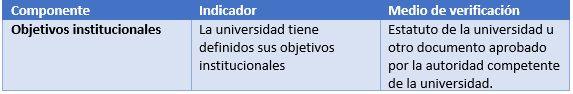
\includegraphics[width=17cm]{./Imagenes/001}
\end{center}	
\vspace{12mm} %5mm vertical space

\textbf{Condición I. Existencia de objetivos académicos, grados y títulos a otorgar y planes de estudio correspondientes.}

Objetivo:
Internalizar en la comunidad universitaria (autoridades, docentes, administrativos y estudiantes) la información que posee y acciones que viene implementando la Universidad Peruana Los Andes con la finalidad de lograr satisfactoriamente su proceso de licenciamiento a través de las ocho condiciones básicas de calidad.\\
Aspecto General del Proceso de Licenciamiento\\
\\
1.	El cumplimiento de las Condiciones Básicas de calidad.\\
2.	Etapas que contempla en proceso de licenciamiento.\\
3.	Otorgar la licencia de funcionamiento institucional a las Universidades.\\
4.	Qué universidades están obligadas a obtener licencia de funcionamiento institucional.\\


\textbf{Condición I: Existencia de objetivos académicos, grados y títulos a otorgar y planes de estudio correspondientes.}\\
-	Según la Ley 30220 y de acuerdo al estatuto de la Universidad Privada de Tacna, reemplazar en sus funcionales del Vicerrectorado Administrativo.\\
-	De acuerdo al estatuto de la Universidad Peruana Los Andes. Propone al Consejo de Facultad la contrata de docentes mediante proceso de selección; 		asimismo la separación en caso de cometer falta grave.\\
-	De acuerdo al estatuto de la Universidad Peruana Los Andes, La universidad se organiza por facultades que son unidades de formación académica, 		profesional y de gestión. Ordene en forma jerárquica: a) Unidades de investigación, b) Los Departamentos Académicos, c) Unidades de posgrado y d) 		Escuelas Profesionales.\\
-	Los estudios generales, los estudios específicos y de especialidad. Tienen una duración mínima de cinco (5) años, los que se realizan en dos semestres     	académicos por año. El enunciado comprende a:\\
-	Para estudios presenciales se define un crédito académico como equivalente a un mínimo de:\\
-	El Plan de estudios de la Escuela Profesional de Administración y Sistemas cumple con los créditos necesarios de pregrado que exige la Ley 30220 para 		el funcionamiento de una carrera, teniendo un total de créditos de: \\
-	El Plan de estudios de la Escuela Profesional de Contabilidad y Sistemas cumple con los créditos necesarios de pregrado que exige la Ley 30220 para el 		funcionamiento de una carrera, teniendo un total de créditos de:\\
-	Los egresados que hayan obtenido el Grado Académico de bachiller pueden obtener el título profesional mediante las siguientes modalidades\\





\section{CONDICION III} 

\vspace{16mm} %5mm vertical space
\begin{center}
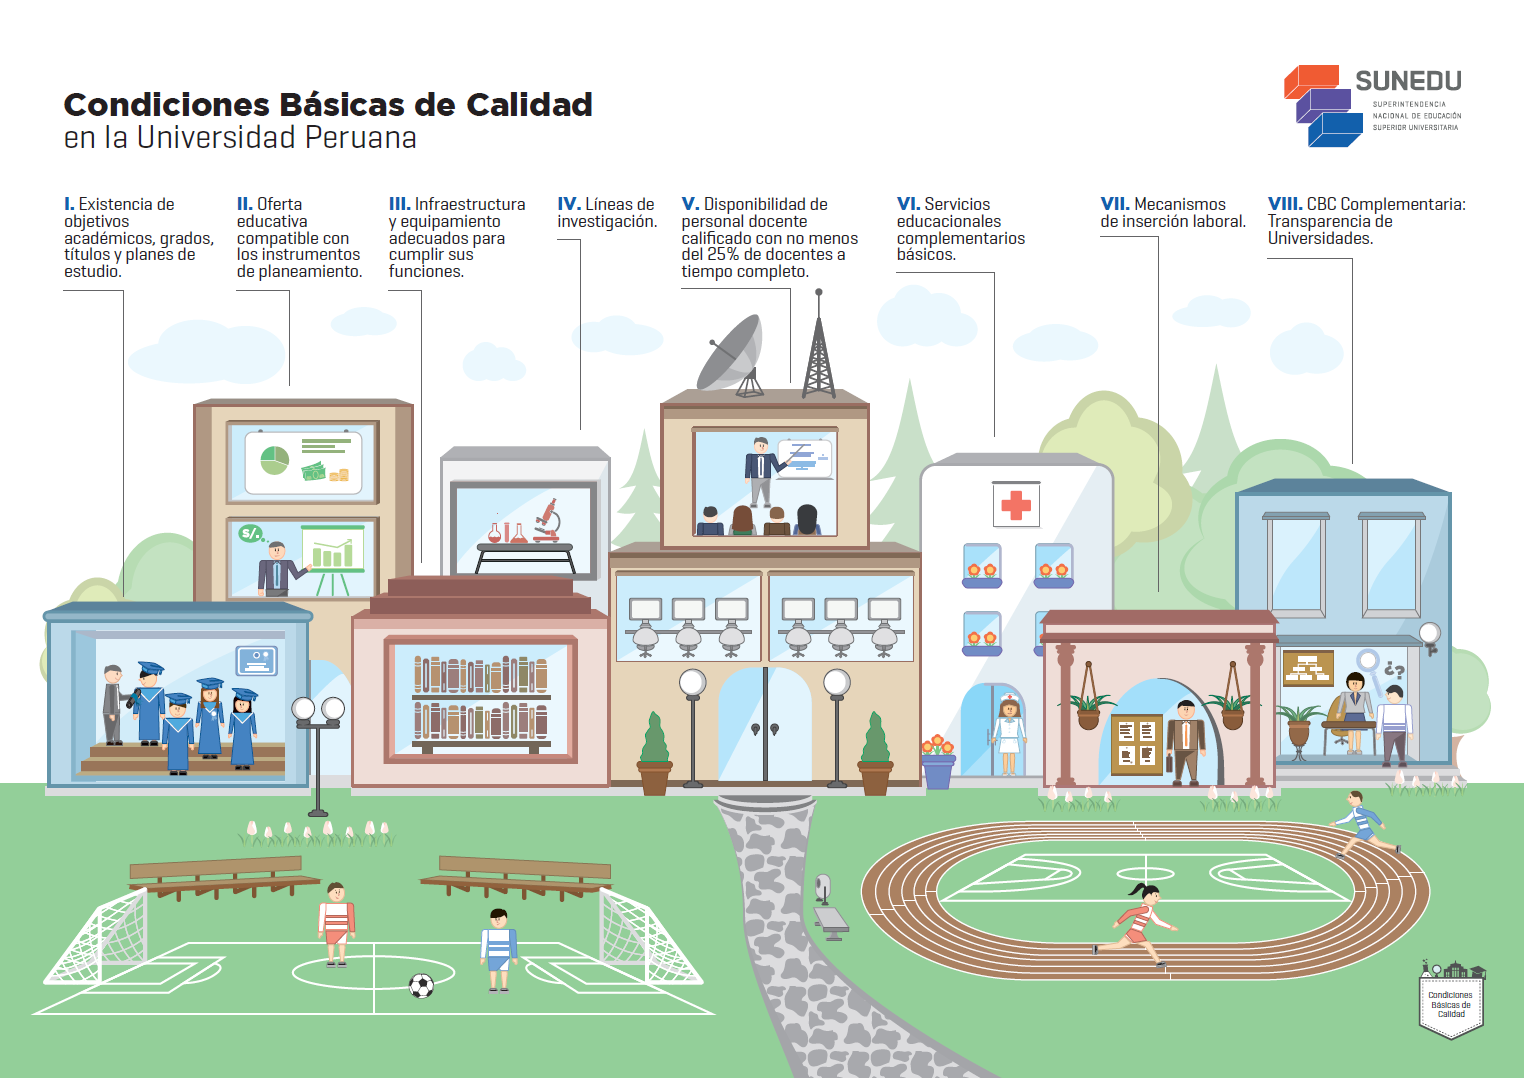
\includegraphics[width=17cm]{./Imagenes/002}
\end{center}	
\vspace{7mm} %3mm vertical space

\textbf{CONDICION III: Infraestructura y equipamiento adecuado al cumplimiento de sus funciones (aulas, bibliotecas, laboratorios, entre otros)}\\
-	ubicación de la FCAC. de acuerdo al certificad o Registral Inmobiliario, y el certificado de numeración de Finca, se encuentra ubicado en: \\
-	Universidad Privada de Tacna con que documentos como medio de verificación acredita la posesión de su local \\
-	El Reglamento interno de seguridad y salud en el trabajo y protocolos de seguridad, que tiene la Universidad Peruana los Andes, mediante qué documento 		ha sido aprobado 17. El Organigrama del comité de Seguridad y Salud en el trabajo que adopto la UPLA. está conformado por\\ 
-	Para el componente III.5 DISPONIBILIDAD DE SERVICIOS PUBLICOS, INDICADOR 21: DISPONIBILIDAD DE AGUA POTABLE Y DESAGÜE, el medio de 			verificación que se acogió la Universidad \\
-	Los ambientes para docentes de acuerdo al medio de verificación MV1: formato de licenciamiento C8, donde se registra información de la ubicación de los 			ambientes para docentes en el local de la universidad.\\


\section{CONDICION IV} 
\textbf{Líneas de investigación a ser desarrolladas}
\vspace{5mm} %5mm vertical space

\vspace{5mm} %5mm vertical space
\begin{center}
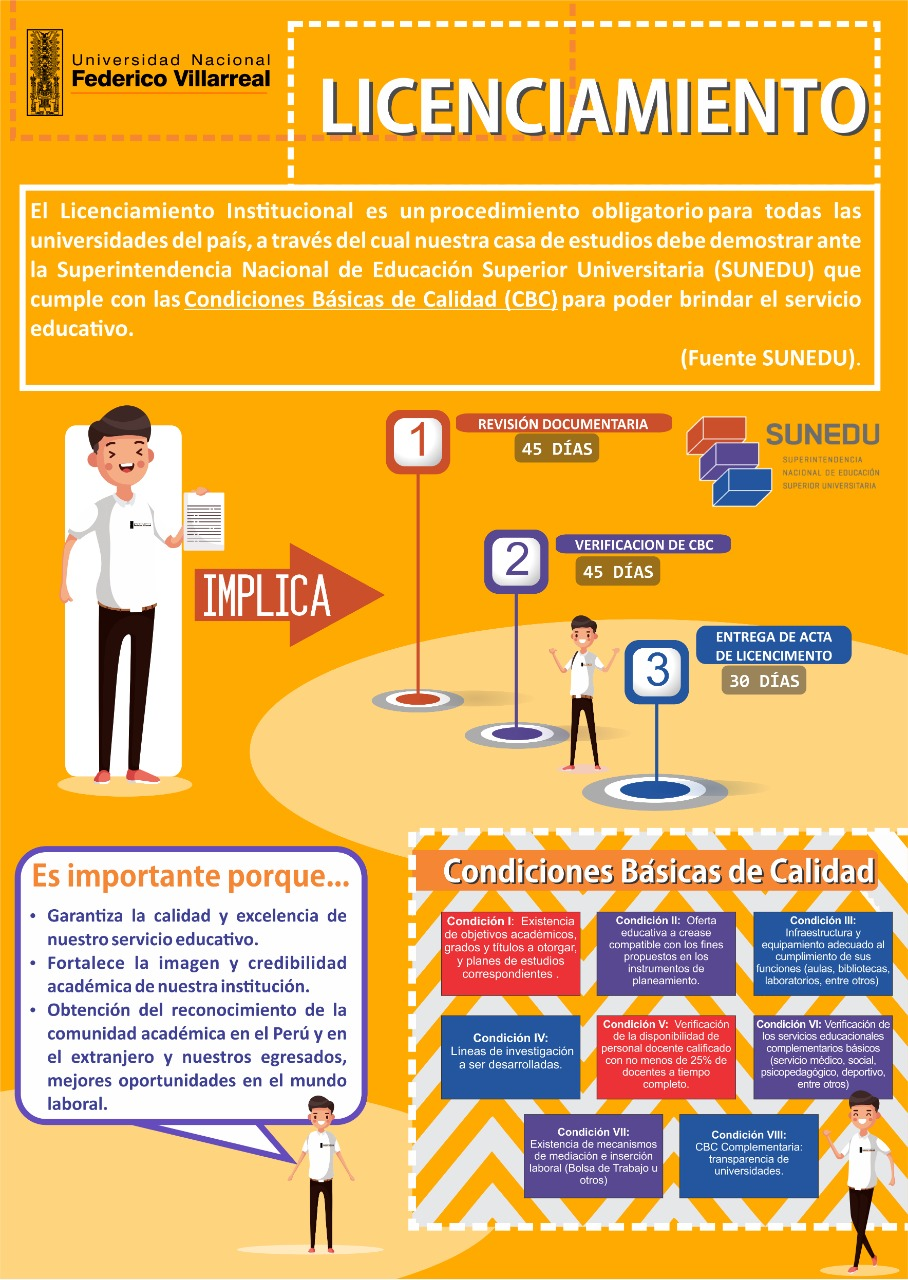
\includegraphics[width=10cm]{./Imagenes/003}
\end{center}	
\vspace{7mm} %3mm vertical space

\textbf{CONDICION IV: Líneas de investigación a ser desarrolladas}\\

-	Son indicadores que corresponden a las líneas de investigación\\
-	Son indicadores que corresponden a docentes que realizan investigación\\ 
-	Son indicadores que corresponden a Registro de documentos y proyectos de investigación.\\
\textbf{CONDICION V: Verificación de la disponibilidad de personal docente calificado con no menos del 25 porciento de docentes a tiempo completo}\\
-	De acuerdo al estatuto vigente de la Universidad Privada de Tacna.\\
\textbf{CONDICION VI: Verificación de los servicios educacionales complementarios básicos (servicio médico, social, psicopedagógico, deportivo, entre otros)}\\
-	Los servicios complementarios básicos con que debe contar mínimamente la universidad son: \\
-	Los servicios complementarios referido a Servicios de salud  \\
-	Los servicios complementarios referido a Servicios culturales  \\
-	Los servicios complementarios referido a Acervo bibliográfico \\
-	Los servicios complementarios referido servicio psicopedagógico\\
 \textbf{CONDICION VII: Existencia de mecanismos de mediación e inserción laboral (Bolsa de Trabajo u otros)}\\
-	Uno de los fines de la Universidad moderna en cuanto a la condición VII\\
-	En la condición VII para que los mecanismos de inserción laboral funcionen\\ 
-	Para el cumplimiento de la condición VII se debe tener en consideración\\
-	La condición VII tiene: CONDICION VIII: CBC complementaria: Transparencia de universidades\\ 
-	Actualmente en el Portal de Transparencia que reglamento(s) de admisión encontramos\\
-         ¿Cuántosi reglamentos de estudiantes actualmente se encuentran en el portal de transparencia?\\ 
-         ¿En el portal de transparencia se encuentran visibles la(s) malla(s) currillar(es) de: \\
-         ¿Cuál es el indicador que corresponde a la Condición Básica de Calidad VIII? \\
-	Es un documento sustentatorio para el medio de verificación MV1 \\
-	Los códigos de los programas de la Escuela Profesional de Contabilidad y Finanzas semipresencial corresponden a:\\ 
-	Los códigos de los programas de la Escuela Profesional de Contabilidad y Finanzas presencial corresponden a: \\
-	Los códigos de los programas de la Escuela Profesional de Administración y sistemas semipresencial corresponden a:\\ 
-	Los códigos de los programas de la Escuela Profesional de Administración y sistemas presencial corresponden a: \\
-	Cuál es el número de cursos generales que tienen los programas de Administración y sistemas – Contabilidad y Finanzas?\







\end{document}
